\begin{frame}{Orientation culturelle (p.~33)}
  \begin{columns}
    \column{0.5\textwidth}
      \begin{minipage}[c][0.6\textheight]{\linewidth}
        \only<1>{
          \small
          Au cours des siècles, les femmes ont joué un rôle social important.
          Néanmoins, pendant longtemps, les droits des femmes ont été limités et ce n'est qu'en 1945 que le droit de vote leur a été accordé en France.
          Aujourd'hui, les femmes et les hommes ont légalement les mêmes droits et peuvent assumer les mêmes responsabilités, grâce aux mouvements féministes des années 70, particulièrement importants pour la libération des femmes.
          Le droit à la contraception et à l'interruption volontaire de grossesse \gloss{pregnancy} (IVG) datent de cette époque.
        }
        \only<2->{
          Outre ces droits acquis du féminisme, de nombreuses études sociologiques, à partir des années 80, se sont penchées sur \gloss{looked at} les différences et les relations entre le genre sexuel, l'orientation sexuelle et le genre social.
          Ces études, appelées <<théorie du genre>>, ne se centrent plus sur les femmes mais sur les distinctions entre homme et femme, en tant que \gloss{as a} construction sociale et culturelle.
        }
      \end{minipage}
    \column{0.5\textwidth}
      \begin{center}
        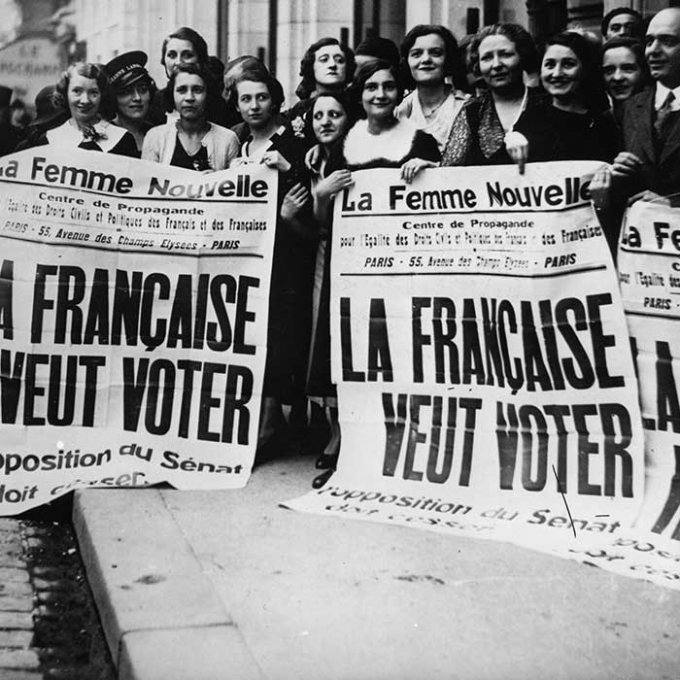
\includegraphics[scale=0.15]{vote.jpg}
      \end{center}
      \only<1>{
        \begin{enumerate}
          \item Quand est-ce que les femmes ont commencé à voter en France?
          \item Est-ce que c'est avant ou après les femmes aux États-Unis?
        \end{enumerate}
      }
      \only<2->{
        \begin{enumerate}
          \setcounter{enumi}{2}
          \item Quelle est une <<construction sociale>>?
          \item Quelle est la théorie du genre?
        \end{enumerate}
        \vspace{0.77cm}
      }
  \end{columns}
\end{frame}